\documentclass[
    12pt,
    a4paper,
    oneside
]{report}

% -------------------------------------------------
% Language and encoding
% -------------------------------------------------

\usepackage[utf8]{inputenc}
\usepackage[T1]{fontenc}
\usepackage[english]{babel}

% -------------------------------------------------
% Page layout and typography
% -------------------------------------------------

\usepackage[
    left=3cm,
    right=2.5cm,
    top=2.5cm,
    bottom=2.5cm
]{geometry}

\usepackage{lmodern}
\usepackage{microtype}
\usepackage{setspace}
\onehalfspacing

% -------------------------------------------------
% Chapter formatting
% -------------------------------------------------

\usepackage{titlesec}

% Roman numerals for the main chapters
\renewcommand{\thechapter}{\Roman{chapter}}

% Display: I Introduction
% Do not display: Chapter I
\titleformat{\chapter}
    {\normalfont\LARGE\bfseries}
    {\thechapter}
    {1em}
    {}

\titlespacing*{\chapter}
    {0pt}
    {-20pt}
    {30pt}

% -------------------------------------------------
% Mathematics
% -------------------------------------------------

\usepackage{amsmath}
\usepackage{amssymb}

% Chapter-relative numbering, for example (IV.1)
\numberwithin{equation}{chapter}

% -------------------------------------------------
% Figures and tables
% -------------------------------------------------

\usepackage{graphicx}
\graphicspath{{figures/}}

\usepackage{booktabs}
\usepackage{tabularx}
\usepackage{longtable}

% Chapter-relative numbering, for example Figure V.2
\numberwithin{figure}{chapter}
\numberwithin{table}{chapter}

% -------------------------------------------------
% Units and source-code excerpts
% -------------------------------------------------

\usepackage{siunitx}

\usepackage{listings}

\lstset{
    basicstyle=\small\ttfamily,
    numbers=left,
    numberstyle=\tiny,
    numbersep=8pt,
    breaklines=true,
    showstringspaces=false
}

% -------------------------------------------------
% Colours
% Required later for documenting AI-assisted content
% -------------------------------------------------

\usepackage{xcolor}

% -------------------------------------------------
% Bibliography
% -------------------------------------------------



% -------------------------------------------------
% Links and cross-references
% -------------------------------------------------

\usepackage[hidelinks]{hyperref}
\usepackage[nameinlink]{cleveref}

% -------------------------------------------------
% Document
% -------------------------------------------------

\begin{document}

% -------------------------------------------------
% Title page
% -------------------------------------------------

\begin{titlepage}

    \begin{center}

        {\LARGE\bfseries Master's Thesis\par}

        \vspace{2.2cm}

        {\LARGE\bfseries
        AI-Based Malaria Diagnosis from Microscopic Thick Blood Smear Images
        \par}

    \end{center}

    \vspace{2.5cm}

    \renewcommand{\arraystretch}{1.5}

    \begin{tabular}{@{}p{4.2cm}p{10cm}@{}}

        Student: &
        Yassine Hermak \\

        Degree Program: &
        Electrical Engineering / Information Technology \\

        Specialization: &
        Information Engineering \\

        First Examiner: &
        Prof. Dr.-Ing. Achim Ibenthal \\

        University: &
        HAWK University of Applied Sciences and Arts
        Hildesheim/Holzminden/Göttingen \\

        Faculty: &
        Faculty of Engineering and Health in Göttingen \\[0.4cm]

        & 
\includegraphics[width=5cm]{HAWK_I_Logo.jpg} \\[0.6cm]

        Second Examiner: &
        Dilane Chanja \\

        In Cooperation With: &
        CarByte Engineering GmbH \\

        Period: &
        July 2026 to November 2026 \\

    \end{tabular}

    \vfill

\end{titlepage}

% -------------------------------------------------
% Front matter
% -------------------------------------------------

\pagenumbering{roman}

\chapter*{Abstract}
\addcontentsline{toc}{chapter}{Abstract}

Malaria detection strongly depends on microscopy and trained personnel, which can limit fast diagnosis and treatment, especially in resource-limited regions where access to such tools may be limited. This work focuses on developing a simpler deep learning approach for malaria prescreening from thick blood smear images, with future deployment using a combination of microscope, ocular adapter and smartphone.

To achieve this goal, the NLM/NIH dataset was used to train and evaluate multiple models based on ResNet50, ResNet18 and MobileNetV3-Small. The task was to classify complete images as either infected or uninfected. Several simulated resolution levels were tested, starting from high resolution at 224 $\times$ 224 pixels down to the lowest resolution of 56 $\times$ 56 pixels. Grad-CAM and Grad-CAM++ were used to analyse which image regions influenced the model predictions.

All architectures showed very high performance at high resolution. The highest accuracy of 99.69\% was achieved by both ResNet18 and MobileNetV3-Small, while ResNet50 achieved 99.58\%. At the lowest reduced resolution, the main decrease was observed in specificity. After a two-stage optimisation, MobileNetV3-Small achieved an accuracy of 92.76\%, a sensitivity of 96.40\%, a specificity of 79.31\% and an F1-score of 95.45\%. Grad-CAM and Grad-CAM++ showed that the models sometimes focused on image borders and dark background areas. To investigate this behaviour further, an external test was performed using the AIR Uganda dataset, which has different image characteristics. ResNet50 and MobileNetV3-Small still detected most infected images at LR3, while ResNet18 showed lower performance.

The achieved results show that MobileNetV3-Small is a promising lightweight model for future deployment. The developed approach is still at the research prototype stage and requires further evaluation before real-world deployment. The next important step is to evaluate the models using real images captured with the microscope, developed ocular adapter and smartphone setup under realistic deployment conditions.


\clearpage
\tableofcontents
\clearpage

% The glossary will be inserted here later.
% According to the HAWK guidance, it should preferably
% appear directly after the table of contents.

% -------------------------------------------------
% Main content
% -------------------------------------------------

\pagenumbering{arabic}

\chapter{Introduction}
\label{chap:introduction}

To this day, malaria continues to pose a major global health challenge. The World Health Organization reports that in 2024, about 282 million people were infected with malaria worldwide, and approximately 610,000 lives were lost to the disease. Among all regions, Africa bears by far the heaviest burden, accounting for the vast majority of cases and deaths. Given these numbers, diagnosing malaria early and accurately is critical, as it allows treatment to begin at the right time, which can help prevent the disease from progressing to severe stages and reduce the risk of death.\cite{WHO2025Malaria}.



\chapter{System Overview}
\label{chap:system-overview}



\chapter{State of Research}
\label{chap:state-of-research}

This chapter provides the background and research basis needed for the development of the diagnostic method. This literature review is a continuation of the work carried out by Kouom Nankam with additional studies that are especially relevant to the focus of this thesis \cite{Kouom2026}. It first introduces the basic medical principles of malaria diagnosis and the main concepts of deep learning that are relevant for this work. Based on this, existing AI-based approaches for malaria diagnosis are reviewed and compared with regard to their data, model types, evaluation methods, and the actual practical use. This chapter starts with the basic medical background of malaria diagnosis and then introduces the deep learning methods that are relevant for this work. After that, previous research approaches are presented and compared. The chapter ends by identifying the main research gap and explaining how it is related to this thesis.

\section{Literature Basis and Previous Work}
\label{sec:literature_basis}

The literature review in this thesis is based on previous work carried out at HAWK Göttingen. In February 2026, Kouom Nankam completed a systematic literature review on AI-based malaria diagnosis using microscopic blood images. His research covered publications from 2022 to 2025 from IEEE Xplore, ScienceDirect, SpringerLink, and PubMed. His search used combinations of terms such as ''malaria diagnosis'', ''deep learning'', ''convolutional neural networks'', ''vision transformer'', and ''microscopic blood smear''. His analysis first began with reviewing the titles and abstracts to check their relevance. After that, the selected studies were read and analysed in full \cite{Kouom2026}.

The review contained 38 references and focused on datasets, preprocessing methods, model architectures, training and validation strategies, evaluation metrics, explainability, and practical applicability. The work was literature-based and did not include its own model implementation or experimental evaluation \cite{Kouom2026}.

Although the review covered different AI approaches for malaria diagnosis, it focused mainly on thin blood smear images. Kouom explicitly excluded thick blood smear analysis from the scope of the work. He pointed out that thick blood smears provide higher sensitivity for parasite detection, but that their complex visual structure and high cell density make automated image analysis and reliable annotation more difficult \cite{Kouom2026}. This limitation is relevant for the present thesis since the diagnostic method developed here focuses specifically on thick blood smear images.

To extend the previous literature review, an additional search was carried out for studies that were directly relevant to the research questions of this thesis. Search terms included combinations of ''malaria'', ''thick blood smear'', ''deep learning'', ''MobileNet'', ''object detection'', ''image resolution'', ''smartphone microscopy'', and ''explainable AI''. The identified studies were reviewed with focus on the parts relevant to this thesis, especially the methods, tools, datasets, and reported results. The findings were then compared with the previous HAWK literature review to avoid unnecessary duplication. Particular attention was given to studies involving thick blood smear images, patient-wise evaluation, reduced image resolution, and explainability.

\begin{table}[htbp]
    \centering
    \caption{Comparison of the HAWK literature review and the literature review of this thesis.}
    \label{tab:literature_review_comparison}
    \begin{tabularx}{\textwidth}{|p{3.2cm}|X|X|}
        \hline
        \textbf{Aspect} & \textbf{Kouom Nankam} & \textbf{This thesis} \\
        \hline
        Literature scope & Publications from 2022--2025 & Previous review extended with additional relevant studies \\
        \hline
        Blood smear type & Mainly thin blood smears. Thick-smear analysis excluded from the review scope & Mainly thick blood smears, thin blood smears included only in the literature review \\
        \hline
        Main focus & General state of AI-based malaria diagnosis & AI-based diagnosis with focus on classification, image resolution, efficiency, and explainability \\
        \hline
        Studies used & 38 references & 35 references including the work of Kouom Nankam\\
        \hline
        Experimental work & No implementation or experiments & Model implementation, training, testing, and benchmarking \\
        \hline
    \end{tabularx}
\end{table}

\FloatBarrier



\section{Malaria and Microscopic Diagnosis}
\label{sec:malaria_microscopy}

Malaria is an infectious disease caused by parasites from the genus Plasmodium. Five species are known to cause malaria in humans: P. falciparum, P. vivax, P. ovale, P. malariae, and P. knowlesi. Among them, P. falciparum is the most dangerous species and is responsible for most deaths caused by severe malaria \cite{Maturana2022}. During the blood stage of the infection, different parasite stages can be seen under the microscope. These include immature trophozoites, also known as ring forms, mature trophozoites, schizonts, and gametocytes \cite{Maturana2022}. These different stages are important for the microscopic diagnosis of malaria.

Giemsa staining is commonly used to make malaria parasites visible in blood smears. The WHO recommends Giemsa staining for both thick and thin blood films \cite{WHO2016Giemsa}. Before staining, the thin blood film is fixed with methanol. The thick blood film should not come into contact with methanol because the red blood cells need to undergo haemolysis. After staining, the slides are rinsed with buffered water and left to dry before they are examined under the microscope \cite{WHO2016Giemsa}.

Two main types of blood smears are used for microscopic malaria diagnosis: thick and thin blood smears. Thick smears are mainly used to check whether malaria parasites are present, while thin smears preserve the structure of the red blood cells and are therefore more suitable for identifying the Plasmodium species \cite{Maturana2022}.

Figure~\ref{fig:thick_thin_smear} shows the visual difference between a thick and a thin Giemsa-stained blood smear.

\begin{figure}[htbp]
    \centering
    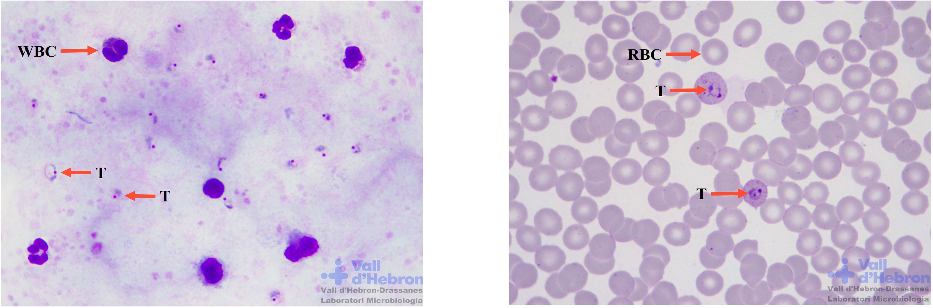
\includegraphics[width=0.8\textwidth]{thin-vs-thick.pdf}
    \caption{Comparison of Giemsa-stained blood smears. The left image shows a thick blood smear and the right image shows a thin blood smear. Source:  Maturana et al. \cite{Maturana2022}.}
    \label{fig:thick_thin_smear}
    \vspace{-0.3cm}
    \end{figure}

\FloatBarrier

In the figure, WBC stands for white blood cells, RBC for red blood cells, and T for trophozoites.

Thick blood smears are more sensitive than thin blood smears and can therefore detect lower parasite levels. Maturana et al. report that thick blood smears are approximately 20 to 40 times more sensitive than thin blood smears \cite{Maturana2022}.

Thin blood smears, on the other hand, keep the individual red blood cells visible. This makes it possible to examine the parasites together with the infected cells and makes species identification easier. The main differences between thick and thin blood smears are shown in Table~\ref{tab:thick_thin_comparison} \cite{Maturana2022}.

\begin{table}[htbp]
    \centering
    \caption{Comparison of thick and thin blood smears for malaria microscopy.}
    \label{tab:thick_thin_comparison}
    \begin{tabularx}{\textwidth}{|p{3.2cm}|X|X|}
        \hline
        \textbf{Aspect} & \textbf{Thick blood smear} & \textbf{Thin blood smear} \\
        \hline
        Main purpose &
        Detection and screening of malaria parasites &
        Identification of the Plasmodium species \\
        \hline
        Sensitivity &
        Higher, reported to be about 20--40 times more sensitive &
        Lower compared with thick smears \\
        \hline
        Red blood cells &
        Broken down during staining &
        Remain intact \\
        \hline
        Parasite visibility &
        Parasites are concentrated in a dense smear area &
        Parasites can be examined inside individual red blood cells \\
        \hline
        Image structure &
        Dense and less clearly structured &
        Individual cells can be seen more clearly \\
        \hline
    \end{tabularx}
\end{table}

\FloatBarrier

Thick blood smears can also be used to estimate the parasite density, not only to detect an infection. For this, the number of parasites is counted together with the number of white blood cells (WBCs). According to the WHO procedure, these values can then be used to calculate the parasite density \cite{WHO2016ParasiteCounting}:

\begin{equation}
D =
\frac{N_P \cdot C_{\mathrm{WBC}}}
     {N_{\mathrm{WBC}}},
\label{eq:parasite_density}
\end{equation}
where $D$ is the estimated parasite density in parasites/$\mu$L, $N_P$ is the number of parasites counted, $N_{\mathrm{WBC}}$ is the number of white blood cells counted, and $C_{\mathrm{WBC}}$ is the patient's white blood cell concentration per $\mu$L.

If the actual WBC concentration is not available, the WHO recommends using an assumed value of 8000 WBC/$\mu$L \cite{WHO2016ParasiteCounting}. Equation~\ref{eq:parasite_density} then becomes

\begin{equation}
D =
\frac{N_P \cdot 8000}
     {N_{\mathrm{WBC}}}.
\label{eq:parasite_density_who}
\end{equation}

Parasite density estimation is not part of the method developed in this thesis. The equations are only included to show how parasite concentration is calculated during conventional microscopic examination. The task of this work focuses instead on classifying thick blood smear images as infected or uninfected.

Although thick blood smears are very sensitive for parasite detection, their image structure makes automatic analysis more difficult. In contrast to thin smears, individual red blood cells are no longer clearly visible, and parasites appear together with other stained blood components and possible artefacts \cite{Yang2020}. Kouom Nankam also describes the complex structure and high cell density of thick smears as challenges for automated image analysis and annotation \cite{Kouom2026}. For this reason, this thesis focuses specifically on the automatic classification of thick blood smear images. Later experiments also investigate how reduced image resolution affects this task.

\section{Deep Learning Fundamentals}
\label{sec:deep_learning_fundamentals}

Since this thesis is based on deep learning, this section introduces the main concepts that are relevant for the developed method. It first explains the basic idea of deep learning and then focuses on convolutional neural networks, transfer learning, image analysis tasks, and the evaluation metrics used later in this work.

\subsection{Convolutional Neural Networks}

{\color{blue}  
A CNN processes an image through several layers. The first layers usually learn simple image features such as edges, colours, and textures. Deeper layers combine these simple features into more complex patterns that are useful for the final prediction \cite{Goodfellow-et-al-2016}. This hierarchical feature extraction is one of the main reasons why CNNs are suitable for image classification.

The main operation of a CNN is the convolution. A small filter, also called a kernel, moves across the input image or feature map and calculates a new feature map. Following the standard formulation of convolution used in deep learning \cite{Goodfellow-et-al-2016}, A simplified two-dimensional convolution operation used in CNNs can be written as:

\begin{equation}
Y(i,j) =
\sum_{m}\sum_{n}
X(i+m,j+n)K(m,n) + b
\label{eq:convolution}
\end{equation}

where $X$ represents the input, $K$ is the convolution kernel, $b$ is a bias term, and $Y$ is the resulting feature map. During training, the values of the kernels are learned automatically from the data.


After a convolution, an activation function is normally applied. A commonly used activation function is the Rectified Linear Unit (ReLU) \cite{Goodfellow-et-al-2016}, which is defined as:

\begin{equation}
\mathrm{ReLU}(x) = \max(0,x)
\label{eq:relu}
\end{equation}


ReLU keeps positive values while setting negative values to zero. This introduces non-linearity and allows the network to learn more complex relationships between the input image and the target class \cite{Goodfellow-et-al-2016}.
}

\begin{tcolorbox}[
    colback=gray!15,
    colframe=gray!50,
    boxrule=0.5pt
]

\textbf{Type and extent of AI use}

Claude was used to extract useful information from the book by Goodfellow et al. The extracted information were used for the deep learning fundamentals section.

\vspace{0.4cm}

\textbf{The individual contribution}

The extracted information were selected based on what was needed for this section and was used according to the structure of the section. The information was then used to explain the main deep learning fundamentals that are relevant to this thesis.

\vspace{0.4cm}

\textbf{Critical evaluation of the AI contribution}

The book by Goodfellow et al. contains more than 800 pages. By using Claude, the relevant information could be found and extracted more efficiently. This also saved time that could be used to analyse other references that are more directly related to the topic of this thesis.

\end{tcolorbox}

The development of CNN architectures has resulted in networks with different levels of complexity. AlexNet demonstrated the potential of deep CNNs for large-scale image classification \cite{Krizhevsky2012}. VGG later increased the network depth using repeated small convolution filters \cite{Simonyan2015}. ResNet introduced residual connections that allow information to bypass individual layers and make the training of deeper networks easier \cite{He2016}. Other architectures focus more strongly on computational efficiency. MobileNet uses depthwise separable convolutions to reduce computational cost \cite{Howard2017}, while SqueezeNet was designed to strongly reduce the number of model parameters \cite{Iandola2016}. These differences between CNN architectures are relevant when selecting a model based not only on classification performance but also on computational requirements.

CNNs are not the only approach used in modern image analysis. Vision Transformers (ViTs) apply the Transformer concept to images by dividing an image into smaller patches and processing the relationships between these patches using attention mechanisms \cite{Dosovitskiy2021}. 

\subsection{Transfer Learning}


Training a deep neural network completely from scratch generally requires a large amount of labelled data. Transfer learning provides an alternative by reusing knowledge learned from another task. In transfer learning, knowledge from a previously learned task is transferred to support learning on a new task \cite{PanYang2010}.

For image classification, pretrained models can be used as a starting point for a new task. The learned features of these models can then be reused for another image classification problem \cite{Rajaraman2018}.

When pretrained models are further trained using a new dataset, this process is commonly referred to as fine-tuning. This approach is also used in malaria image analysis, for example by Maturana et al., who fine-tuned pretrained detection models using their thick blood smear dataset \cite{Maturana2023}.

{\color{blue}  
During training, the model parameters are updated by minimising a loss function. For classification tasks, cross-entropy loss is commonly used to measure the difference between the predicted class probabilities and the true class label \cite{Goodfellow-et-al-2016}. For a classification problem with \(C\) classes, the cross-entropy loss can be written as:

\begin{equation}
L = -\sum_{c=1}^{C} y_c \log(p_c)
\label{eq:cross_entropy}
\end{equation}

where \(y_c\) represents the true class label and \(p_c\) the predicted probability for class \(c\).

During model development, the available data are normally separated into training, validation, and test data. The training set is used to update the model parameters. The validation set is used to observe the model during development and to support decisions such as model or hyperparameter selection. The test set should remain separate and is used for the final evaluation of the trained model. This separation is important because evaluating the model on data that were already used during training can lead to an unrealistic estimation of its performance \cite{Goodfellow-et-al-2016}.
}

\begin{tcolorbox}[
    colback=gray!15,
    colframe=gray!50,
    boxrule=0.5pt
]

\textbf{Type and extent of AI use}

Claude was used to extract useful information from the book by Goodfellow et al. The extracted information was used for the deep learning fundamentals section.

\vspace{0.4cm}

\textbf{The individual contribution}

The extracted information was selected based on what was needed for this section and was arranged according to the structure of the chapter. It was then used to explain the main deep learning fundamentals that are relevant to this thesis.

\vspace{0.4cm}

\textbf{Critical evaluation of the AI contribution}

The book by Goodfellow et al. contains more than 800 pages. By using Claude, the relevant information could be found and extracted more efficiently. This also saved time that could be used to analyse other references that are more directly related to the topic of this thesis.

\end{tcolorbox}

\subsection{Image Analysis Tasks}

The studies reviewed in this thesis use different image analysis tasks. The main tasks relevant to this work are classification, object detection, and segmentation.

Image classification assigns a class to an image or image region. For example, a binary classifier can distinguish between infected and uninfected samples \cite{Rajaraman2018}. However, classification does not show where an object is located in the image.

Object detection also identifies the position of objects, usually using bounding boxes. YOLO is a common example of an object detection approach \cite{Redmon2016}. In malaria analysis, this can be used to locate individual parasites or blood cells.

Image segmentation works at pixel level and assigns a label to individual pixels \cite{Kassim2021RBCNet}. This allows structures such as cells or background regions to be separated more precisely.

Since these tasks solve different problems, their results and evaluation metrics should not be compared directly without considering the task being performed.

\subsection{Evaluation Metrics}

The performance of a binary classification model can be described using true positives ($TP$), true negatives ($TN$), false positives ($FP$), and false negatives ($FN$). In this thesis, infected samples are treated as the positive class and uninfected samples as the negative class. The following evaluation metrics are based on these values \cite{Delahunt2024}:

\begin{equation}
\mathrm{Accuracy} =
\frac{TP+TN}
{TP+TN+FP+FN}.
\label{eq:accuracy}
\end{equation}

Sensitivity, also called recall, describes how many infected samples are correctly identified:

\begin{equation}
\mathrm{Sensitivity} =
\mathrm{Recall} =
\frac{TP}
{TP+FN}.
\label{eq:sensitivity}
\end{equation}

Specificity describes how many uninfected samples are correctly identified:

\begin{equation}
\mathrm{Specificity} =
\frac{TN}
{TN+FP}.
\label{eq:specificity}
\end{equation}

Precision describes how many samples predicted as infected are actually infected:

\begin{equation}
\mathrm{Precision} =
\frac{TP}
{TP+FP}.
\label{eq:precision}
\end{equation}

The F1-score combines precision and recall:

\begin{equation}
F_1 =
2 \cdot
\frac{\mathrm{Precision}\cdot\mathrm{Recall}}
{\mathrm{Precision}+\mathrm{Recall}}.
\label{eq:f1_score}
\end{equation}

These metrics describe different parts of the model performance. Sensitivity is especially important for showing how reliably infected samples are detected, while specificity shows how reliably uninfected samples are identified \cite{Delahunt2024}.

The Receiver Operating Characteristic (ROC) curve shows the relationship between the true-positive rate and false-positive rate at different classification thresholds. The Area Under the ROC Curve (ROC-AUC) summarises this behaviour in one value. Delahunt et al. point out that metrics such as ROC-AUC and F1 should be interpreted carefully in malaria diagnosis and emphasise the importance of patient-level evaluation \cite{Delahunt2024}.

Object detection studies can also report Average Precision (AP) or mean Average Precision (mAP). These metrics are relevant to the object detection studies discussed later in this chapter, but they are not used to evaluate the classifiers developed in this thesis.

\section{AI-Based Malaria Diagnosis from Microscopic Images}
\label{sec:ai_malaria_diagnosis}

Automated malaria diagnosis has developed from traditional image-processing methods towards deep learning-based approaches. Earlier methods often used manually designed image features, while more recent approaches use convolutional neural networks to learn relevant features directly from microscopic images \cite{Maturana2022,Quinn2016}.

The literature includes different tasks such as image classification, parasite detection, species identification, and patient-level diagnosis. Kassim et al., for example, combined parasite detection and classification to distinguish between P. falciparum, P. vivax, and uninfected samples at image and patient level \cite{Kassim2021}.

Both thin and thick blood smear images have been used for automated malaria analysis. Thick blood smears are especially relevant for parasite screening, but their dense image structure makes automatic analysis more difficult \cite{Maturana2022}. For this reason, the following sections focus mainly on approaches using thick blood smear images.

Smartphone-based microscopy has also become relevant for automated malaria diagnosis. Quinn et al. used CNNs for malaria detection from thick blood smear images captured using smartphones \cite{Quinn2016}. Such approaches are relevant to this thesis because the future system is also intended to combine a microscope, smartphone, and automated image analysis.

\section{Thick Blood Smear Datasets and Image Acquisition}
\label{sec:datasets_acquisition}

For the practical work of this thesis, three thick blood smear datasets were considered: the datasets provided by the National Library of Medicine (NLM), the Uganda dataset presented by Quinn et al., and the Drassanes--Vall d'Hebron dataset.

The NLM provides thick blood smear images from patients infected with P. falciparum and P. vivax, as well as images from uninfected patients. Yang et al. published a dataset containing 1819 images from 150 patients infected with P. falciparum. The images were captured using a smartphone camera connected to a microscope and contain 84 961 manually annotated parasites \cite{Yang2020}. Kassim et al. later used a combined NLM collection containing 5972 images from 350 patients with P. falciparum, P. vivax, and uninfected samples \cite{Kassim2021}.

The Uganda dataset presented by Quinn et al. contains 1182 thick blood smear images with 7245 annotated parasites \cite{Quinn2016}. The images were captured using a smartphone microscope setup. Since the dataset contains malaria-positive images and parasite-level annotations, it is mainly suitable for parasite detection rather than infected-versus-uninfected classification. In this thesis, it was later used as an external test dataset.

The Drassanes--Vall d'Hebron dataset contains 2571 labelled thick blood smear images \cite{VallHebron2025}. The images were captured using either a Leica microscope camera or a Samsung Galaxy S20 connected to the microscope. The dataset contains different Plasmodium species and object-level annotations. However, all included thick blood smear samples are malaria-positive, which means that the dataset cannot directly provide an uninfected class for the binary classification task used in this thesis.

Table~\ref{tab:malaria_datasets} gives an overview of the three datasets.

\begin{table}[htbp]
    \centering
    \caption{Overview of the thick blood smear datasets considered in this thesis.}
    \label{tab:malaria_datasets}
    \begin{tabularx}{\textwidth}{|p{2.7cm}|X|X|X|}
        \hline
        \textbf{Dataset} &
        \textbf{Size} &
        \textbf{Acquisition} &
        \textbf{Main characteristics} \\
        \hline

        NLM datasets &
        5972 images / 350 patients reported by Kassim et al. &
        Smartphone microscopy &
        P. falciparum, P. vivax, and uninfected samples \cite{Yang2020,Kassim2021} \\
        \hline

        Uganda / AIR &
        1182 images / 7245 annotated parasites &
        Smartphone-microscope setup &
        Malaria-positive thick smear images with parasite-level annotations \cite{Quinn2016} \\
        \hline

        Drassanes--Vall d'Hebron &
        2571 labelled images &
        Leica microscope camera or Samsung Galaxy S20 &
        Multiple Plasmodium species and object-level annotations; malaria-positive samples \cite{VallHebron2025} \\
        \hline

    \end{tabularx}
\end{table}

\FloatBarrier

The NLM datasets were selected for the main training and internal evaluation because they contain both infected and uninfected patients. The P. falciparum and P. vivax images could therefore be combined into one infected class and compared with the uninfected class.

The high original image resolution was also useful for the resolution experiments in this thesis because lower-resolution versions could be generated from the same images. The final dataset preparation, class definition, patient-wise splitting, and preprocessing are described in Chapter~\ref{chap:implementation}.

\section{CNN-Based Classification Approaches}
\label{sec:cnn_classification}

CNNs are widely used for automated malaria image classification because they can learn relevant image features directly from the training data. Different approaches have used pretrained CNNs, custom CNN architectures, or a combination of detection and classification.

Rajaraman et al. investigated pretrained CNNs for the classification of parasitized and uninfected cells in thin blood smear images \cite{Rajaraman2018}. The evaluated architectures included AlexNet, VGG-16, ResNet-50, Xception, and DenseNet-121. The study showed that features learned by pretrained CNNs can be reused for malaria image classification.

For thick blood smears, Yang et al. developed a method that combines Iterative Global Minimum Screening (IGMS) with a custom CNN \cite{Yang2020}. IGMS first selects possible parasite candidates from the microscopic image. The CNN then classifies the extracted patches as parasite or background. Their CNN achieved an accuracy of 93.46\%, a sensitivity of 92.59\%, and a specificity of 94.33\%. The study is particularly relevant because it uses smartphone-acquired thick blood smear images. However, the classification is performed on selected image patches instead of the complete microscopic image.

Kassim et al. also combined detection and classification for thick blood smear images \cite{Kassim2021}. Their PlasmodiumVF-Net first detects parasite candidates using Mask R-CNN and then uses ResNet50 to reduce false-positive detections. The final system provides decisions at image and patient level and distinguishes between P. falciparum, P. vivax, and uninfected samples. This study is especially relevant because it uses the same NLM dataset family that is used in this thesis.

These studies show that CNNs can be used in different ways for malaria analysis. Rajaraman et al. used pretrained CNNs for cell classification, while Yang et al. and Kassim et al. combined candidate detection with CNN-based classification. In contrast, this thesis investigates direct binary classification of complete thick blood smear images without a separate parasite detection step.

ResNet50 and ResNet18 are used as the main residual architectures in this thesis. Lightweight architectures such as MobileNet are discussed separately in Section~\ref{sec:lightweight_networks}.

\section{Object Detection Approaches}
\label{sec:object_detection}

Object detection is used when individual parasites or blood cells need to be located inside a microscopic image. Unlike image classification, the model does not only predict a class but also identifies the position of the detected objects. This is mostly useful in malaria analysis because several parasites can appear within the same microscopic field.

Maturana et al. investigated object detection on thick blood smear images as part of the iMAGING system \cite{Maturana2023}. They compared YOLOv5x, Faster R-CNN, SSD, and RetinaNet using a dataset of 2571 labelled images. The models detected leukocytes, early trophozoites, and mature trophozoites. YOLOv5x achieved a precision of 92.10\%, a recall of 93.50\%, an F-score of 92.79\%, and an mAP@0.5 of 94.40\%. This study is particularly relevant because it combines thick blood smear analysis with smartphone-based image acquisition and automated microscopy.

Vásquez Ascate et al. developed a smartphone-based object detection system for thick blood smears \cite{VasquezAscate2026}. Their dataset contained 8625 images from 400 slides captured using three different smartphones. Several lightweight object detection models were evaluated. YOLOv11n achieved an accuracy of 90.92\% and an F1-score of 93.8\%. The study is relevant to this thesis because it combines thick blood smears, smartphone image acquisition, and models designed for mobile deployment.

These studies show that object detection can be used to locate individual parasites inside thick blood smear images. However, this requires object-level annotations and a different processing approach than the method used in this thesis. The present work instead focuses on binary classification of the complete image as infected or uninfected without directly locating individual parasites.

\section{Lightweight Networks and Computational Efficiency}
\label{sec:lightweight_networks}

For this thesis, classification performance is not the only important point. The computational requirements of a model are also important because the final system is intended for deployment with limited resources. A smaller model can be more suitable for limited hardware even if its accuracy is slightly lower than that of a larger model.

The MobileNet family was developed for efficient image processing on mobile and embedded devices \cite{Howard2017}. MobileNet reduces the computational cost by using depthwise separable convolutions instead of standard convolutions. This makes the architecture smaller and more efficient while still allowing useful image features to be learned.

Lightweight models are also relevant in recent malaria research. Vásquez Ascate et al. evaluated several lightweight object detection models for smartphone-based analysis of thick blood smear images \cite{VasquezAscate2026}. Their work shows the importance of model size and computational efficiency when malaria analysis is intended for mobile devices.

In this thesis, MobileNetV3-Small is used as the lightweight alternative to ResNet50 and ResNet18. The objective is to investigate whether a smaller model can still achieve good classification performance, especially when the image resolution is reduced. This is relevant for the future system because the model should not only perform well, but should also remain suitable for practical deployment.

\section{Influence of Image Resolution}
\label{sec:image_resolution}

Image resolution is important in this thesis because malaria parasites can appear as small structures inside a microscopic image. When the resolution is reduced, some visual details can be lost, which may affect the performance of the model.

In the studies reviewed for this thesis, image resolution is usually defined by the dataset or the image acquisition setup. Yang et al., for example, used smartphone-acquired thick blood smear images with an original resolution of 3024~$\times$~4032 pixels \cite{Yang2020}. Their method detects possible parasite regions and then classifies smaller image patches. However, different resolution levels were not compared systematically.

Kassim et al. also used high-resolution smartphone images from the NLM thick blood smear datasets \cite{Kassim2021}. Their work focuses on parasite detection and malaria classification, but does not investigate how the model performance changes when the image resolution is reduced.

This leaves an open question about how much image detail can be reduced before the classification performance begins to decrease. This is relevant for the system developed in this project because the final images will be captured using a microscope, ocular adapter, and smartphone, and their image characteristics may differ from the original dataset images.

For this reason, this thesis investigates several controlled resolution levels using the same thick blood smear images. This makes it possible to study how the loss of image detail affects whole-image classification while keeping the underlying image content and patient data unchanged.

\section{Explainability in Malaria Diagnosis}
\label{sec:explainability}

Deep learning models can achieve high classification performance, but it is often difficult to understand which parts of an image influenced the prediction. In medical image analysis, this is important because the model should focus on relevant image regions instead of unrelated structures or background information.

Rajaraman et al. investigated this problem for malaria classification using thin blood smear images \cite{Rajaraman2018Explainability}. They used different visualisation methods, including saliency maps, occlusion sensitivity, class activation maps, and Grad-CAM. Their results showed that the trained CNNs focused on regions containing malaria parasites.

Grad-CAM uses the gradients of a predicted class to create a heatmap showing which regions of the image contributed most to the prediction \cite{Selvaraju2017}. In this thesis, Grad-CAM and Grad-CAM++ are used to inspect true-positive, true-negative, false-positive, and false-negative predictions.

This helps to investigate whether the models focus on relevant regions inside the microscopic field or on unrelated areas such as image borders or background.

\section{Comparison of Relevant Approaches}
\label{sec:comparison_approaches}

The studies reviewed in the previous sections use different datasets, tasks, and evaluation methods. Their reported results therefore cannot be compared directly. Table~\ref{tab:comparison_relevant_approaches} gives a short overview of the thick blood smear studies that are most relevant to this thesis.

\begin{table}[htbp]
\centering
\small
\caption{Comparison of selected thick blood smear approaches.}
\label{tab:comparison_relevant_approaches}

\begin{tabularx}{\textwidth}{|p{2.5cm}|X|X|X|X|}
\hline
\textbf{Study} &
\textbf{Data} &
\textbf{Task} &
\textbf{Approach} &
\textbf{Reported Results} \\
\hline

Yang et al. \cite{Yang2020} &
1819 images from 150 patients &
Parasite candidate classification &
Candidate screening + custom CNN &
93.46\% accuracy, 92.59\% sensitivity, 94.33\% specificity \\
\hline

Kassim et al. \cite{Kassim2021} &
5972 images from 350 patients &
Parasite detection and image/patient classification &
Mask R-CNN + ResNet50 &
83.9\% image-level accuracy, 92.3\% patient-level accuracy \\
\hline

Maturana et al. \cite{Maturana2023} &
2571 labelled images &
Parasite and leukocyte detection &
YOLOv5x, Faster R-CNN, SSD, RetinaNet &
YOLOv5x: 92.79\% F-score, 94.40\% mAP@0.5 \\
\hline

Vásquez Ascate et al. \cite{VasquezAscate2026} &
8625 images from 400 slides &
Parasite detection &
Several lightweight object detection models &
YOLOv11n: 90.92\% accuracy, 93.8\% F1-score \\
\hline

\end{tabularx}
\end{table}

\FloatBarrier

The comparison shows that the studies use different approaches for thick blood smear analysis. Yang et al. classify selected parasite candidates, while Kassim et al. combine parasite detection with image- and patient-level classification. Maturana et al. and Vásquez Ascate et al. focus mainly on locating parasites inside the image.

The studies also show the importance of smartphone-based image acquisition and models that can be used with limited resources. However, the tasks are different, so their reported performance values should not be compared directly.

Another difference is that the reviewed studies mainly work with the image resolution provided by their dataset or acquisition setup. The effect of systematically reducing the image resolution is not the main focus of these studies.

\section{Research Gap and Relevance to This Thesis}
\label{sec:research_gap}

The reviewed studies show that different approaches are used for automated malaria analysis. Yang et al. first select possible parasite regions from thick blood smear images and then classify the extracted patches \cite{Yang2020}. Kassim et al. also use a multi-stage approach that combines parasite detection with further classification \cite{Kassim2021}. In contrast, this thesis investigates binary classification of the complete thick blood smear image as infected or uninfected without locating individual parasites.

Another important point is image resolution. The thick-smear studies of Yang et al. and Kassim et al. use images with a fixed original resolution \cite{Yang2020,Kassim2021}. The influence of systematically reducing the image resolution is not the main focus of these studies, but it is relevant for the planned system because the images will later be captured using a microscope, ocular adapter, and smartphone, and their image characteristics may differ from the original dataset images.

Explainability is also relevant for this work. Rajaraman et al. showed that Grad-CAM can be used to inspect which regions influence malaria classification \cite{Rajaraman2018Explainability}. In this thesis, Grad-CAM and Grad-CAM++ are used to investigate whether the models focus on relevant regions inside the microscopic image or on unrelated areas such as image borders or background.

Based on these points, this thesis compares ResNet50, ResNet18, and MobileNetV3-Small using the same dataset and preprocessing conditions. The models are evaluated at different simulated resolution levels to investigate how the loss of image detail affects classification performance. MobileNetV3-Small is also included as a lightweight alternative for future deployment with limited resources.

The main focus of this thesis is therefore the combination of whole-image thick-smear classification, reduced image resolution, different CNN architectures, and explainability. These points form the basis for the method development and experiments described in the following chapters.evaluation, and explainability. These findings provide the basis for the requirements defined in the following chapter.

\chapter{Requirements Analysis}
\label{chap:requirements-analysis}



\chapter{Concept Development}
\label{chap:concept-development}

This chapter converts the findings from the literature review in Chapter~\ref{chap:state-of-research} and the requirements defined in Chapter~\ref{chap:requirements-analysis} into concrete structural decisions for the AI-based classification system.

This section of the thesis explains the background behind selecting the CNN architectures, the processing pipeline, the training strategy, the hyper-parameter selection, the evaluation setup, and the Grad-CAM analysis.

These decisions establish the basis for the implementation described in the next chapter which is Chapter~\ref{chap:implementation}.

\section{Selection of CNN Architectures}

Three CNN architectures were selected for this thesis: ResNet50, ResNet18, and MobileNet. The selection was based on two main factors from the literature review: classification performance and computational efficiency.

Since classification performance is an important objective of this work, ResNet50 and ResNet18 were selected as the main residual architectures. As discussed in Section~\ref{sec:cnn_classification}, Rajaraman et al. \cite{{Rajaraman2018} evaluated several CNN architectures for malaria cell classification using patient-level cross-validation. ResNet50 achieved high classification performance compared with the other tested architectures. ResNet18 was added as a smaller ResNet variant to investigate whether a less complex residual network can achieve comparable classification performance.

MobileNet was selected as the lightweight architecture for the intended system. As discussed in Section~\ref{sec:lightweight_networks}, lightweight CNN architectures are useful when computational resources are limited, which is relevant to this project. MobileNet reduces computational effort by using depth-wise separable convolutions and is therefore suitable for comparing classification performance with a more efficient network design. This is important for the intended PC-based diagnostic system and also for possible future deployment where computational resources are limited.

The three architectures were therefore selected to represent two different goals. ResNet50 and ResNet18 focus more on classification performance, while MobileNet represents the lightweight side of the comparison. This addresses the two aspects of the research gap identified in Section~\ref{sec:research_gap}: achieving strong classification performance while also considering computational efficiency.

\section{Processing Pipeline}

The processing pipeline describes how a thick blood smear image is transformed from the original input into a classification result. It represents the AI-related part of the overall system introduced in Chapter~\ref{chap:system-overview}.

The overall processing pipeline is shown in Figure~\ref{fig:processing_pipeline}.

\begin{figure}[htbp]
    \centering
    \fbox{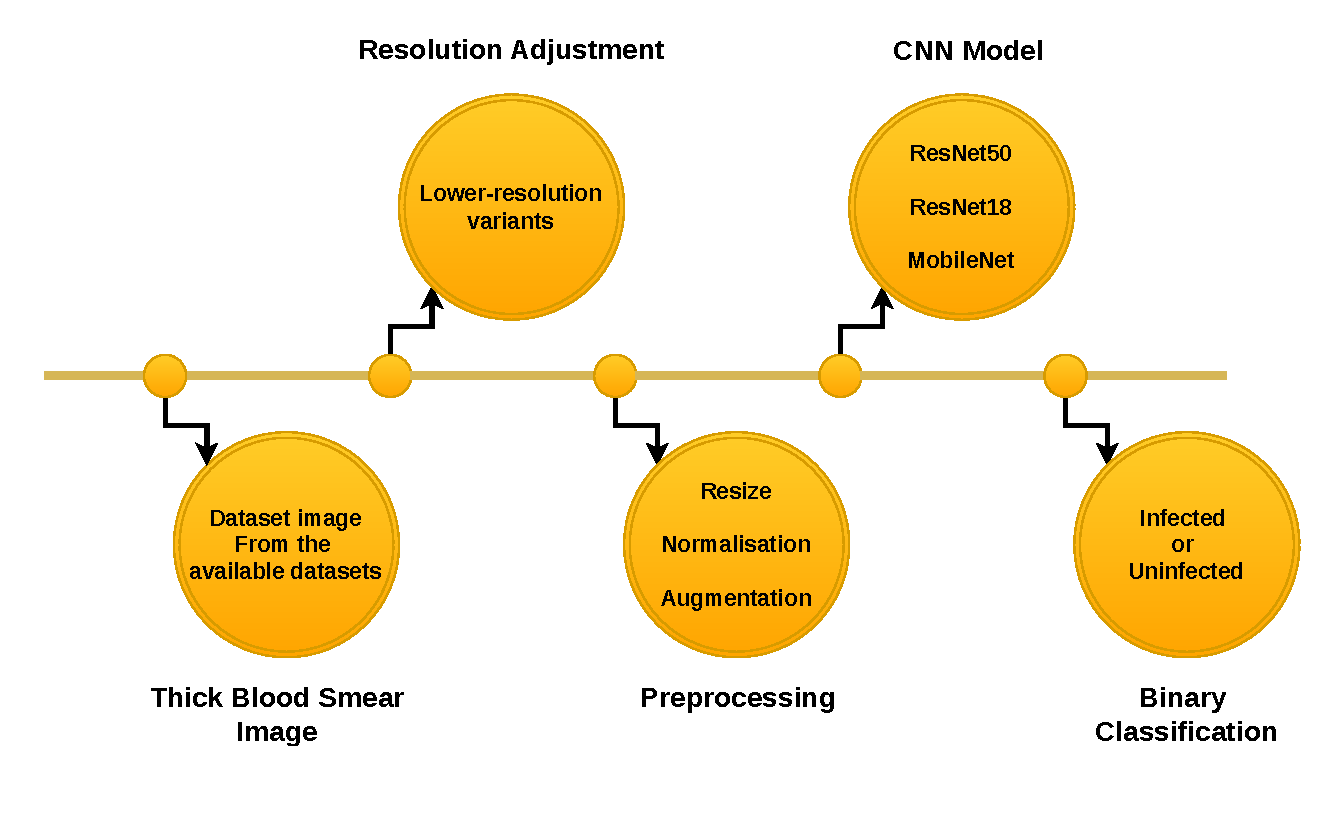
\includegraphics[width=0.9\textwidth]{Processing_Pipeline.pdf}}
    \caption{Processing pipeline of the AI-based malaria classification system.}
    \label{fig:processing_pipeline}
\end{figure}

\FloatBarrier

A complete thick blood smear image is used as an input for classification, without detecting parasite regions or identifying parasite types. The goal is to classify each image as either infected or uninfected, which is the main goal of this thesis. This differs from many of the reviewed approaches in chapter~\ref{chap:state-of-research}, which first extract parasite regions or cell-level areas before classification.

Before the image is passed to the CNN model, preprocessing is applied. This includes normalisation and resizing to the input size required by the selected architecture. During training, data augmentation is also used.

For the resolution experiments, the same source images are processed at different resolution levels in separate runs. The image is first reduced to the selected lower resolution and is then resized to the input size expected by the model. This makes it possible to compare how the same architecture behaves under different image resolutions.

The preprocessed image is then passed through one of the selected CNN architectures: ResNet50, ResNet18, or MobileNet. The model produces a binary classification result predicting whether the image is infected or uninfected.

\section{Training Strategy}
\label{sec:training_strategy}

The selected CNN models are trained using transfer learning. To save time and computing power, pretrained ImageNet weights are used as the starting point for the models. The models are then fine-tuned using the malaria thick blood smear images. This approach makes it possible for the networks to start from already learned image features and adapt them to the task of malaria classification.

The final classification layer is adapted to two output classes: infected and uninfected. Cross-entropy loss, explained in Section~\ref{sec:deep_learning_fundamentals}, is used during the training to show how wrong the model’s prediction is compared with the correct class. Adam is then used as the optimiser for updating the model parameters during training. The same training strategy is applied to ResNet50, ResNet18, and MobileNet in order to keep the comparison between the architectures more fair.

To support model generalisation, data augmentation is applied only to the training images. The augmentation includes horizontal and vertical flipping as well as small image rotations. The goal is to increase the variation of the training data and reduce the risk of overfitting. The validation images are not augmented.

During training, the validation accuracy is calculated after each epoch. Each time a higher validation accuracy is reached, the corresponding checkpoint is saved. If the same validation accuracy is reached again, the previously saved checkpoint is kept. The checkpoint with the highest validation accuracy is later used for the final test evaluation.

\section{Hyperparameter Selection}

The hyperparameters were selected based on the available hardware. Since the training was performed on a MacBook Pro with an M2 chip and 8 GB of memory, moderate settings were chosen to keep the training stable and manageable.

The same main hyperparameters were used initially for ResNet50, ResNet18, and MobileNet. A learning rate of 0.0001, which is suitable for fine-tuning pretrained models, was used together with the Adam optimiser. The batch size was set to 8, and each model was trained for 15 epochs. The pretrained networks were fine-tuned as complete models rather than keeping the earlier layers frozen.

Using the same training parameters for all three architectures makes the comparison more reliable by reducing the effect of different hyperparameter settings on the results. It is also planned that, if one of the lightweight models shows very low performance, an additional optimisation may be carried out. This approach was also discussed within the project team and was considered suitable for a fair comparison of the selected architectures.

After each epoch, the validation accuracy was calculated, and the checkpoint with the highest validation accuracy was saved for later evaluation.

\begin{table}[htbp]
\centering
\caption{Main hyperparameters used for training.}
\label{tab:hyperparameters}
\begin{tabularx}{\textwidth}{|p{5cm}|X|}
\hline
\textbf{Hyperparameter} & \textbf{Selected value} \\
\hline
Learning rate & 0.0001 \\
\hline
Batch size & 8 \\
\hline
Number of epochs & 15 \\
\hline
Optimizer & Adam \\
\hline
Weight initialization & pretrained on ImageNet\\
\hline
Fine-tuning & Complete network \\
\hline
Model selection & Highest validation accuracy \\
\hline
\end{tabularx}
\end{table}

\FloatBarrier

\section{Evaluation Setup}

The evaluation is constructed to compare the selected CNN architectures for this work under the same conditions and to investigate how reduced image resolution affects the classification performance.

The high-resolution baseline uses an image size of \(224 \times 224\) pixels, which corresponds to the standard input size used by the pretrained ResNet and MobileNet models. For the reduced resolution experiments, the same source images are reduced to lower resolutions (LR1/LR2/LR3) and then resized back to \(224 \times 224\) pixels before being given to the CNN model. In this way, the input size of the network stays unchanged while the amount of image detail is reduced. The lowest tested resolution is \(56 \times 56\) pixels and represents the extreme low-resolution case.

The dataset is divided into training, validation, and test sets using a standards patient-based split of 70\%, 15\%, and 15\%. All images belonging to the same patient remain in the same subset. This avoids using images from the same patient for both training and evaluation.

The classification performance is evaluated using accuracy, sensitivity, specificity, precision, F1-score, and ROC-AUC. These metrics were already explained in Section~\ref{sec:deep_learning_fundamentals}. Using several metrics makes it possible to evaluate the overall classification accuracy as well as the behaviour of the models for infected and uninfected images.

The experiments are carried out in several steps. First, a high-resolution baseline is established. The influence of reduced image resolution is then investigated using lower-resolution runs of the same images. At the end, the selected CNN architectures are compared under the defined evaluation conditions. This approach reduces the number of unnecessary training runs while allowing the influence of image resolution to be investigated.

\captionsetup[table]{skip=2pt}
\begin{table}[htbp]
\centering
\caption{Resolution levels used in the evaluation.}
\label{tab:resolution_levels}
\begin{tabularx}{\textwidth}{|p{3cm}|X|}
\hline
\textbf{Resolution level} & \textbf{Image size} \\
\hline
HR & 224$\times$224 pixels \\
\hline
LR1 & 160$\times$160 pixels \\
\hline
LR2 & 112$\times$112 pixels \\
\hline
LR3 & 56$\times$56 pixels \\
\hline
\end{tabularx}
\end{table}

\FloatBarrier

\section{Grad-CAM Analysis}

During the test phase, Grad-CAM is used to understand the behaviour of models that show weak performance. As discussed in Section~\ref{sec:explainability}, Grad-CAM generates a heatmap that highlights the image regions that have the strongest influence on a prediction.

The analysis is therefore focused on underperforming cases, for example models or resolution settings with lower classification performance. The goal here is to investigate whether the model still focuses on meaningful regions inside the microscopic image, for example areas containing parasites, or whether the prediction is influenced by unrelated areas such as the background or image edges.

Grad-CAM is also applied to some selected true-positive, true-negative, false-positive, and false-negative predictions. This makes it possible to compare successful and incorrect classifications and to better understand how the model behaves in different prediction cases.

The Grad-CAM analysis is used as a supporting method together with the evaluation metrics. This helps to identify reasons for unusual model behaviour that cannot be explained by accuracy, sensitivity, specificity, or F1-score alone. The generated heatmaps are presented and discussed in the evaluation chapter.

\chapter{Implementation}
\label{chap:implementation}

In this chapter, it is described how the AI-based malaria classification system was implemented based on the concept developed in Chapter~\ref{chap:concept-development}. It explains the dataset used for the implementation, the preprocessing pipeline, the software tools (such as PyTorch, torchvision and Matplotlib), and the structure of the developed pipeline.
This chapter also explains how the individual components (dataset loading, preprocessing, training, testing and Grad-CAM Analysis) are connected and how reproducibility is supported through fixed data splits, saved model checkpoints, and version-controlled development.

\section{Data Acquisition}

The image data used for the implementation was obtained from publicly available malaria microscopy datasets. No new blood smear images were collected as part of this thesis. 

The training, validation, and main evaluation were based on the NLM/NIH thick blood smear dataset, which has also been used by Kassim et al. \cite{Kassim2021}. It was decided that the NLM/NIH dataset was the perfect match for the developed model because it contains thick blood smear images from infected and uninfected patients, which means it fits the binary classification task of this thesis. Another important advantage is its patient-based structure, which makes it easy to separate the data at patient level and avoid images from the same patient appearing in both training and evaluation sets.

Two additional public datasets were considered during the dataset selection. The Uganda microscopy dataset described by Quinn et al. \cite{Quinn2016} contains thick blood smear images with parasite annotations and is more suitable for parasite detection and localisation tasks. This dataset is available for download on the official website of AIR Uganda which belongs to Makerere University. The Uganda dataset was later used only for an external test of the trained models to check whether the predictions depend strongly on dataset-specific image characteristics. The second dataset is the Vall d'Hebron dataset \cite{VallHebron2025} which also contains labelled thick blood smear images, but mainly provides malaria-positive samples. This one is also not suitable for the infected-versus-uninfected classification used in this work. To get access to this dataset, an application was submitted, and access to the dataset was granted afterwards. 

The Vall d'Hebron dataset was obtained as a possible data source for a future extension of the project, for example towards parasite detection or species identification.

No image data from the Ethiopian Artificial Intelligence Institute were available for the implementation of this thesis. The developed AI method and the other components of the overall project are intended to be transferred to EAII for later development and testing.

\section{Dataset Description}
\label{sec:dataset-description}

As explained in the previous section, the NLM dataset is the most suitable dataset for this work. It consists of three thick blood smear subsets which contain images from uninfected patients, patients infected with Plasmodium vivax, and patients infected with Plasmodium falciparum. All these three subsets contain Giemsa-stained thick blood smear images acquired through the eyepiece of a microscope at 100$\times$ magnification using a smartphone camera. The original images are RGB images with a resolution of 3024 $\times$ 4032 pixels \cite{Yang2020,Kassim2021}.

The uninfected subset contains 1141 images from 50 malaria-negative patients \cite{Kassim2021}. The images are stored in TIFF format and are organised in separate folders by patient. The dataset also provides annotations for white blood cells, which are not needed for the whole-image classification used in this thesis.

 The P. vivax subset contains images from 150 malaria-infected patients, with approximately 20 images per patient \cite{Kassim2021}. Kassim et al. report in their paper a total of 3013 images, while 3014 images were found in the downloaded dataset and used in the implementation. The images are stored in JPEG format and parasite locations are provided in separate annotation files. Since the goal of this thesis is to classify complete images rather than identify individual parasites, these parasite annotations were also not used for the classification process.

The P. falciparum subset contains images from 150 infected patients, with approximately 12 images per patient \cite{Yang2020}. Yang et al. report a total of 1819 images, while 1883 images were found in the downloaded dataset and used in the implementation. These images are also stored in JPEG format. The corresponding annotation files contain information about parasite and white blood cell positions. Just like the P. vivax subset, these annotations were not required for the whole-image classification task.

For the classification task, the two infected subsets were combined into one positive class. Images from patients infected with P. vivax or P. falciparum were assigned to the class infected, while the images from the uninfected subset were assigned to the class uninfected. In total, 6038 images were included in the implementation: 1141 uninfected images, 3014 P. vivax images, and 1883 P. falciparum images. The final classification task therefore contains two output classes: infected and uninfected.

In addition to the NLM dataset, the Uganda microscopy dataset was used as an external test dataset \cite{Quinn2016}. It contains 1182 malaria-positive images stored in JPEG format. The dataset does not provide patient IDs, and all images used for this external evaluation were assigned to the test split. The Uganda dataset was kept completely separate from the training and validation process and is therefore not included in the 6038 NLM images described above.

\section{Data Preprocessing Pipeline}
\label{sec:data-preprocessing}

Before diving into training the model, the raw data must first be prepared in a way that makes it readable and consistent. This section walks through the preprocessing steps used in this work.

The preprocessing pipeline was implemented in the following steps: First, the image information and binary labels were prepared using the script \textbf{build\_labels.py}. The images were then loaded using the \textbf{MalariaDataset} class from the \textbf{dataset.py} script. After that, the required preprocessing transforms were applied for training, validation, and testing. These transforms are different depending on the split. Training images received random augmentation, while validation and test images did not. For the low-resolution experiments, the same images were reduced to the selected resolution before being resized back to \(224 \times 224\) pixels, which is the required input resolution for the model.

The script \textbf{build\_labels.py} goes through all three NLM image folders for \textbf{Uninfected}, \textbf{P. vivax}, and \textbf{P. falciparum} images. The binary labels are assigned based on the images folder. Images from the uninfected subset receive label 0, while images from both infected subsets receive the same label 1. As mentioned in Section~\ref{sec:dataset-description}, the parasite and white blood cell annotation files provided with the dataset are not used, since the classification in this thesis is based on the complete image.

A file named \textbf{labels.csv} is generated by this script, which stores  the following information for every image: the image path, the class, the binary label, the patient ID, and the assigned dataset split. The split used here is a conventional split using 70\,\% of the patients for training, 15\,\% for validation, and 15\,\% for testing with a random seed of 42. The output is 4186 training images, 899 validation images, and 953 test images.

This generated labels file is then read by the \textbf{MalariaDataset} class in \textbf{dataset.py}. This class selects the images based on the chosen split (train, validation or test) and also adds the stored path from the CSV file to the main dataset path. Each image is then opened by PIL (Pillow) and converted to RGB format. The binary label is read directly from the generated CSV file. This class does not define the resizing, augmentation, or normalisation steps. The transform chain is passed to the class from the training or testing script.

For the high-resolution experiment, no additional resolution reduction is needed. This means, the original images are resized directly to \(224 \times 224\) pixels before being given to the CNN model. During training, random horizontal and vertical flips are used with a probability of 0.5. In addition, random rotations between \(-15^\circ\) and \(+15^\circ\) are also applied. After the augmentation, the image is converted to a numerical format (PyTorch tensor) and normalised using the ImageNet mean and standard deviation values. These preprocessing steps are defined directly in the \textbf{train.py} script.

The same preprocessing pipeline is performed on the low-resolution experiments, with an additional resizing process before the augmentation. The image is first resized to the resolution defined for the experiment and is then resized back to \(224 \times 224\) pixels. LR1 uses \(160 \times 160\) pixels, LR2 uses \(112 \times 112\) pixels, and LR3 uses \(56 \times 56\) pixels. The final input size of the CNN remains \(224 \times 224\) pixels for all resolutions.

The tested resolution levels are summarised in Table~\ref{tab:resolution_levels}.

\begin{table}[htbp]
    \centering
    \caption{Resolution levels used in the experiments.}
    \label{tab:resolution_levels}
    \begin{tabular}{|l|c|c|}
        \hline
        \textbf{Resolution level} & \textbf{Reduced resolution} & \textbf{CNN input size} \\ \hline
        HR  &  No reduction
        & \(224 \times 224\) \\ \hline
        LR1 & \(160 \times 160\) & \(224 \times 224\) \\ \hline
        LR2 & \(112 \times 112\) & \(224 \times 224\) \\ \hline
        LR3 & \(56 \times 56\) & \(224 \times 224\) \\ \hline
    \end{tabular}
\end{table}

\FloatBarrier

To avoid confusion, these low-resolution images are not images that were originally captured at these resolutions. Instead, the lower-resolution conditions are simulated from the same NLM dataset images. The images are first reduced and then resized back to \(224 \times 224\) pixels. In short, the network input size remains unchanged while image details are reduced. 

The Figure~\ref{fig:resolution_comparison} shows an example of the difference between the HR and LR3 conditions.

\begin{figure}[htbp]
    \centering
    \fbox{
        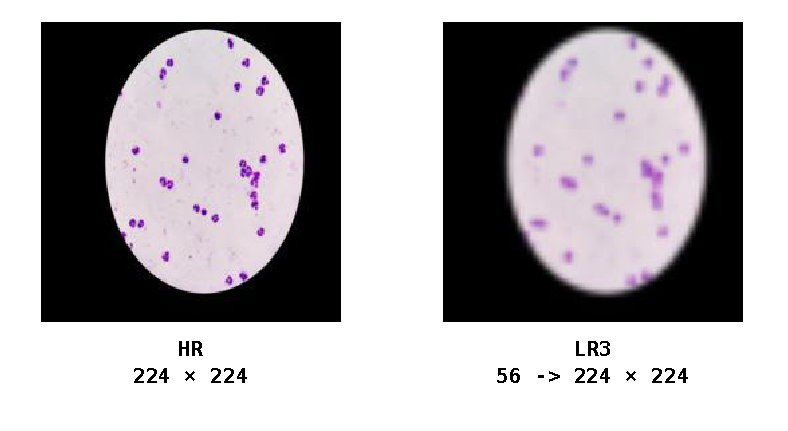
\includegraphics[width=0.68\textwidth]{figures/hr_lr3_comparison.pdf}
    }
    \caption{Example of the same thick blood smear image from patient folder \textbf{PvTk1} under the HR and LR3 resolution conditions.}
    \label{fig:resolution_comparison}
\end{figure}

\FloatBarrier

Keeping this preprocessing step simple was also important. As a result, the resolution reduction was implemented directly in the preprocessing pipeline.

\begin{lstlisting}[
    language=Python,
    caption={Resolution reduction used for the LR3 experiment.},
    label={lst:lr3_resize},
    xleftmargin=0.18\textwidth,
    xrightmargin=0.18\textwidth,
    frame=single
]
transforms.Resize((56, 56)),
transforms.Resize((224, 224)),
\end{lstlisting}

The same implementation is used for LR1 and LR2 by replacing the reduced resolution with \(160 \times 160\) pixels and \(112 \times 112\) pixels.

For validation and testing, no random augmentation is used. In the HR experiment, the images are only resized to \(224 \times 224\) pixels, converted to tensors, and normalised. In the case of a low-resolution experiment, the same resolution reduction used during training is also applied to the validation and test images before resizing them back to \(224 \times 224\) pixels. After that, the images are converted to tensors and normalised. This means that the same resolution condition is used for training, validation, and testing, while the random flips and rotations are only used during training to keep the results reliable.

For the external test with the Uganda dataset, the images were processed using the same LR3 test transform, first resized to \(56 \times 56\) pixels and then resized back to \(224 \times 224\) pixels. The already trained models were used directly without any retraining.

\section{Software Stack and Tools}

This work was developed in Python 3.12.2 and executed through the macOS Terminal. PyTorch was used as the main deep learning framework to build, train, and test the CNN models. Additionally, the torchvision library provided the pretrained network architectures (ResNet50, ResNet18 and MobileNetV3-Small) and also the image preprocessing transforms.

The microscope images were loaded by Pillow(PIL), while pandas read and handled the \textbf{labels.csv} file. The NumPy library managed the numerical operations, and to evaluate the developed models, scikit-learn was used to calculate metrics such as the confusion matrix, classification report, and ROC-AUC score. Matplotlib created the training curves, confusion matrices, and ROC curves.

When it comes to understanding how some models behave, the \textbf{pytorch-grad-cam} library plays a big role. It was used to generate Grad-CAM and Grad-CAM++ visualisations, which show which regions the model is concentrating on while making a prediction.

The scripts were also prepared to run directly from the Terminal. The Python \textbf{argparse} module is responsible for passing settings such as the dataset path, number of epochs, batch size, learning rate, and checkpoint folder as command-line arguments. The \texttt{--data-root} argument replaced the dataset path that was previously written directly in the script. This made the script more flexible, since it can be used with different dataset locations or on another computer without changing the path inside the Python file.

\begin{lstlisting}[
    language=Python,
    caption={Command-line arguments used in the training script.},
    label={lst:argparse},
    xleftmargin=0.10\textwidth,
    xrightmargin=0.10\textwidth,
    basicstyle=\ttfamily\small\color{blue},
    keywordstyle=\color{blue}\bfseries,
    commentstyle=\color{blue},
    stringstyle=\color{blue},
    identifierstyle=\color{blue}
]
def get_args():
    parser = argparse.ArgumentParser()
    parser.add_argument("--data-root", type=str, required=True)
    parser.add_argument("--labels-csv", type=str, default="labels.csv")
    parser.add_argument("--epochs", type=int, default=15)
    parser.add_argument("--batch-size", type=int, default=8)
    parser.add_argument("--lr", type=float, default=0.0001)
    parser.add_argument("--checkpoint-dir", type=str,
                        default="checkpoints")
    return parser.parse_args()
\end{lstlisting}

\begin{tcolorbox}[
    colback=gray!15,
    colframe=gray!50,
    boxrule=0.5pt
]

\textbf{Type and extent of AI use}

 \texttt{argparse} was first seen on some Kaggle competitions inside a python script. The idea sounded useful and Claude was then asked to create a similar function based on the
variables used in this work. Using the –data-root argument was also suggested by Claude instead of keeping the dataset path fixed inside the script.  Both were added to this project.

\vspace{0.4cm}

\textbf{The individual contribution}

The function was then integrated into the training script with the parameters that were used for the experiments, such as dataset path, epochs, batch size, learning rate, and checkpoint folder. 
The fixed dataset path was replaced with the \texttt{--data-root} argument.

\vspace{0.4cm}

\textbf{Critical evaluation of the AI contribution}

The \texttt{argparse} function is not necessary for the model, because the values could also be written directly in the script. But it made the work more flexible because the settings can be changed from the Terminal without going into the Python file every time. The \texttt{--data-root} argument was especially useful because the same script can now be used with a different dataset location without changing the source code.
\end{tcolorbox}

The training and testing scripts also include an automatic device selection. The scripts first check if a CUDA-supported GPU is available. If not, they check for the Apple MPS backend, and if neither is available, the CPU is used. Since the experiments in this work were executed on the MacBook Pro M2, the MPS backend was selected. The automatic device-selection logic was adapted from an example found on the PyTorch Forums.\footnote{\url{https://discuss.pytorch.org/t/same-model-gets-slightly-different-results-on-different-platforms/194551}, accessed 24 July 2026.}

\begin{lstlisting}[
    language=Python,
    caption={Automatic device selection adapted from a PyTorch Forum example.},
    label={lst:device_selection},
    xleftmargin=0.18\textwidth,
    xrightmargin=0.18\textwidth
]
if torch.cuda.is_available():
    device = torch.device("cuda")
elif torch.backends.mps.is_available():
    device = torch.device("mps")
else:
    device = torch.device("cpu")

print("using device:", device)
\end{lstlisting}

A GitHub repository was also created to make access to the model architectures and scripts easy for all team members, serving as a platform for version control, source code storage, and project updates.

The software versions used during the implementation are shown in Table~\ref{tab:software_versions}.

\begin{table}[htbp]
    \centering
    \caption{The software and library versions used in the implementation.}
    \label{tab:software_versions}
    \begin{tabular}{|l|l|}
        \hline
        \textbf{Software / Library} & \textbf{Version} \\ \hline
        Python & 3.12.2 \\ \hline
        PyTorch & 2.13.0 \\ \hline
        torchvision & 0.28.0 \\ \hline
        pandas & 2.2.2 \\ \hline
        NumPy & 1.26.4 \\ \hline
        Pillow & 10.4.0 \\ \hline
        scikit-learn & 1.5.1 \\ \hline
        Matplotlib & 3.10.0 \\ \hline
        pytorch-grad-cam & 1.5.5 \\ \hline
    \end{tabular}
\end{table}

\FloatBarrier

\section{Pipeline Architecture and Integration}
\label{sec:pipeline-architecture}


The implementation of the classification model is made of separate scripts, where each script is responsible for a specific stage of the overall pipeline. The pipeline consists of \textbf{build\_labels.py}, \textbf{dataset.py}, \textbf{train.py}, \textbf{test.py}, and \textbf{gradcam.py}. Keeping these scripts separated made it easier to reuse the same parts of the pipeline for different network architectures and also for reduced resolutions.

The pipeline starts with the NLM dataset folders, which offer a clean separation of the two classes (one folder for uninfected and 2 folders for infected: P. vivax and P. falciparum). The first script is \textbf{build\_labels.py} that goes through the three image folders and creates the \textbf{labels.csv} file. This CSV file stores the image path, class, binary label, patient ID, and the assigned dataset split. These generated information are then used by the \textbf{MalariaDataset} class in the second script which is \textbf{dataset.py}. This \textbf{MalariaDataset} class links the information from the CSV file to the actual image files and then loads the requested split (training, validation, or test).

The \textbf{dataset.py} script does not contain the preprocessing for the specific experiments. Instead, the preprocessing transforms are provided to the \textbf{MalariaDataset} class from the training or testing script. This means that the same dataset class can be reused for the HR, LR1, LR2, and LR3 experiments by only changing the corresponding transform pipeline.

During training, \textbf{train.py} loads the training and validation data through the defined \textbf{MalariaDataset} class. After that, the chosen CNN is configured for binary classification and trained with the given hyperparameters. After every epoch, the model is also evaluated on the validation set. After each validation step, the model is saved as \textbf{best\_model.pth} if its accuracy outperforms all previous epochs. This model represents the best model found during the training process.

After training, \textbf{test.py} loads the same CNN architecture used in training and the saved \textbf{best\_model.pth} checkpoint. The fixed test split is used for the final evaluation. During testing, the model parameters are not changed. The script calculates the evaluation metrics (accuracy, sensitivity, specificity, precision, f1-score and ROC-AUC) and also creates outputs such as the confusion matrix and ROC curve.

The main connection between the scripts and the generated files is shown in Figure~\ref{fig:implementation_pipeline}. The external test was not included in the figure because it uses a separate dataset and a separate testing script and does not form part of the main NLM training, validation, and testing pipeline.

\begin{figure}[htbp]
    \centering
    \fbox{
        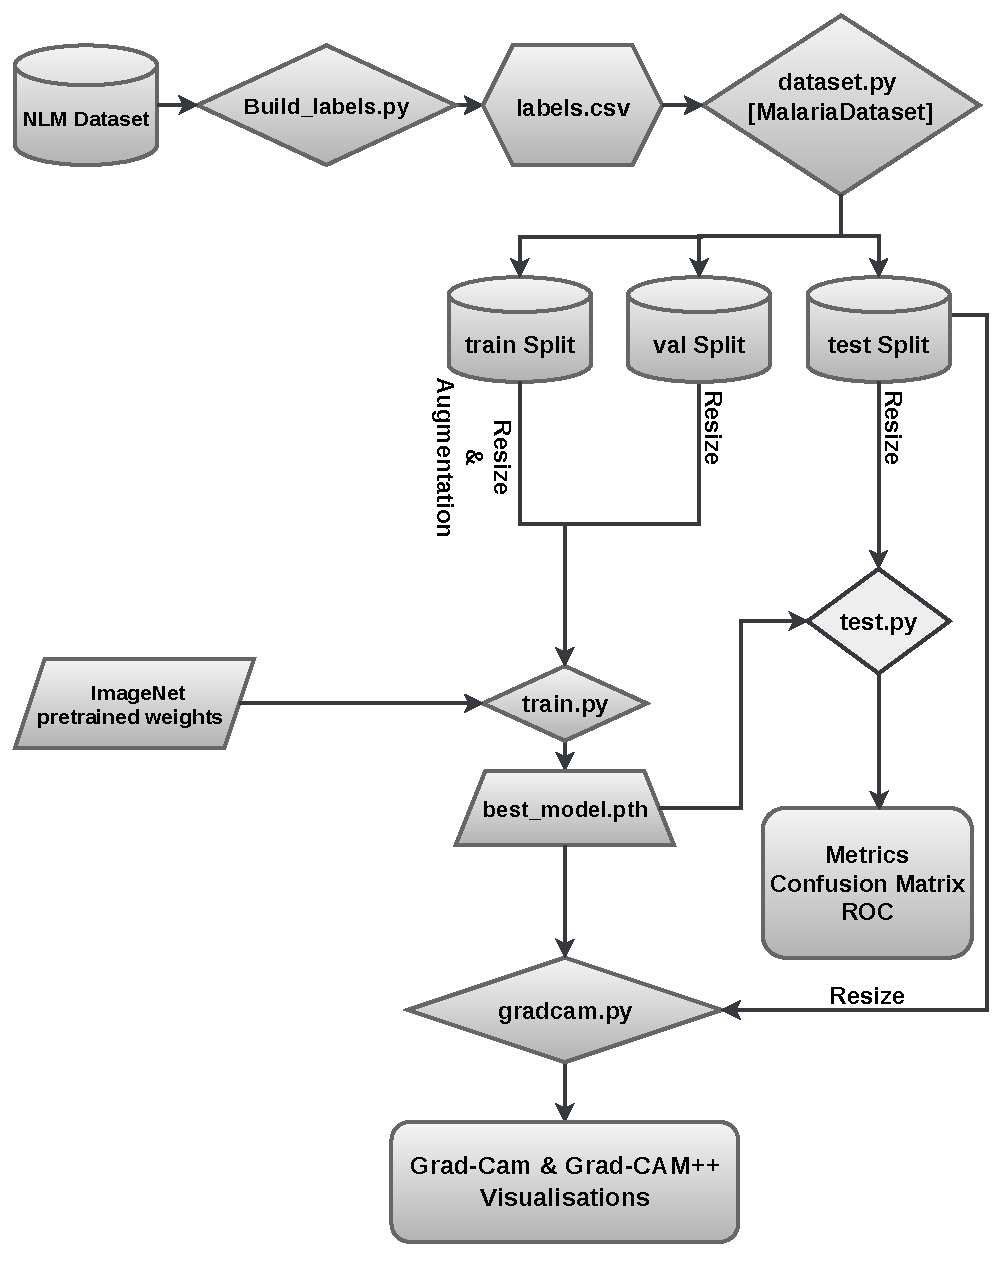
\includegraphics[width=0.85\textwidth]{figures/implementation_pipeline.pdf}
    }
    \caption{Script and data flow of the implemented classification pipeline.}
    \label{fig:implementation_pipeline}
\end{figure}

\FloatBarrier

For the external test, the same testing process was reused with a separate \textbf{labels\_uganda.csv} file and the script \textbf{test\_uganda.py}. The Uganda images were kept separate from the main NLM pipeline and were only used with already trained checkpoints, without any additional training or optimisation.

The last analysis step is conducted by \textbf{gradcam.py}. This script loads the already trained checkpoint from the training and uses images selected from the test set to generate Grad-CAM and Grad-CAM++ visualisations. In the \textbf{gradcam.py} script, the test predictions are first separated into true positive, true negative, false positive, and false negative groups. A limited number of examples from these groups are then used for the explainability analysis. The generated heatmaps are saved as image files for later visual evaluation and also for documentation purposes.

To keep the completed experiments separated from each other, each experiment was stored in its own folder together with the corresponding scripts and also the generated outputs. This made it easier to return to an older experiment without changing its original settings or results. It also helped when comparing the different architectures and resolution conditions. Furthermore, this separation allowed the team members to access the finished experiments without any complication.

The number of experiments was not the same for all three network architectures. ResNet50 was trained and tested at all four resolution conditions: HR, LR1, LR2, and LR3. ResNet18 and MobileNetV3-Small were trained and tested only at HR and LR3. This resulted in a total of eight main experiment runs. The different experiment runs are shown in Table~\ref{tab:experiment_coverage}.

\begin{table}[htbp]
    \centering
    \caption{Experiment runs for the three CNN architectures.}
    \label{tab:experiment_coverage}
    \begin{tabular}{|l|c|c|c|c|}
        \hline
        \textbf{Architecture} & \textbf{HR} & \textbf{LR1} & \textbf{LR2} & \textbf{LR3} \\ \hline
        ResNet50 & Yes & Yes & Yes & Yes \\ \hline
        ResNet18 & Yes & No & No & Yes \\ \hline
        MobileNetV3-Small & Yes & No & No & Yes \\ \hline
    \end{tabular}
\end{table}

\FloatBarrier

After completing the four resolution experiments with ResNet50, only two resolutions (HR and LR3) were selected for the comparison with ResNet18 and MobileNetV3-Small. These two conditions represent the two ends of the tested resolution range. HR represents the normal input condition, while LR3 with \(56 \times 56\) pixels represents the highest simulated resolution reduction used in this work. This made it possible to compare the three architectures under normal and strongly reduced image quality without repeating all four resolution experiments for every architecture.

The LR3 condition is relevant to the planned use of the model together with the smartphone-based ocular adapter. However, the \(56 \times 56\) pixel resolution is not a measured resolution of the final adapter. It was used only as a simulated worst-case resolution to investigate the behaviour of the models when the image detail is extremely reduced. 

Even though performance degraded across all architectures at LR3, the drop in specificity was the most obvious. Because MobileNet is lightweight and more suitable for future deployment, it was decided to optimise only this model. The original performance metrics for ResNet18 and ResNet50 were preserved as baseline comparisons.

The LR3 experiment on MobileNetV3-Small was then performed in three stages. The first stage used the same settings as the other architectures (ResNet50 and ResNet18): a learning rate of \(0.0001\), a batch size of 8, and 15 epochs. The training behaviour of this configuration was unstable.

For the first optimisation, the learning rate was reduced to \(0.00003\), the batch size was increased to 16, and the number of epochs was also increased to 30. These changes resulted in more stable training. After this optimisation, the classification was still not balanced enough between the two classes. That is why a second optimisation was performed by keeping the previous settings from the first optimisation and additionally adding class weights of \([2.0, 1.0]\) for the uninfected and infected classes. This made errors on the uninfected class have a higher influence on the training loss.

The three MobileNetV3-Small configurations are summarised in Table~\ref{tab:mobilenet_optimisation}.

\begin{table}[htbp]
    \centering
    \caption{MobileNetV3-Small configurations used for the LR3 experiment.}
    \label{tab:mobilenet_optimisation}
    \begin{tabular}{|l|c|c|c|c|}
        \hline
        \textbf{Configuration} & \textbf{Learning rate} & \textbf{Batch size} & \textbf{Epochs} & \textbf{Class weights} \\ \hline
        Baseline & 0.0001 & 8 & 15 & None \\ \hline
        Optimisation 1 & 0.00003 & 16 & 30 & None \\ \hline
        Optimisation 2 & 0.00003 & 16 & 30 & [2.0, 1.0] \\ \hline
    \end{tabular}
\end{table}

\FloatBarrier

This optimisation was deliberately limited to MobileNetV3-Small. As already discussed in Chapter~\ref{chap:concept-development}, the ResNet models are mainly used as stronger reference architectures for comparing classification performance, while MobileNet is more relevant for lightweight deployment. Re-optimising all three architectures was therefore outside the scope of this work. The numerical results of all experiments and the results of the MobileNet optimisations are presented later in Chapter~\ref{chap:testing}.

\section{Reproducibility}

The source code of the project is maintained in a GitHub repository and is available at \url{https://github.com/H-Yassine/malaria-diagnosis-master-thesis.git}.

The final version of the implementation used in this thesis corresponds to commit \textbf{\url{https://github.com/H-Yassine/malaria-diagnosis-master-thesis/commit/b256db2}}. The repository history contains \textbf{24 commits}, which document the development of the implementation between july 2026 and october 2026. In addition to the source code, the repository contains a \textbf{meetings/} folder where presentation files and project updates from the regular meetings were kept. The image datasets themselves are not distributed through the repository. The repository therefore provides only the code and pipeline structure, while the original datasets have to be obtained separately from their corresponding sources.

The structure of the repository is shown in Figure~\ref{fig:github_structure}. The project files are separated into four main folders: data, meeting documents, thesis files, and implementation scripts. Every experiment folder is stored inside the scripts folder of the repository.

\begin{figure}[htbp]
    \centering
    \fbox{
        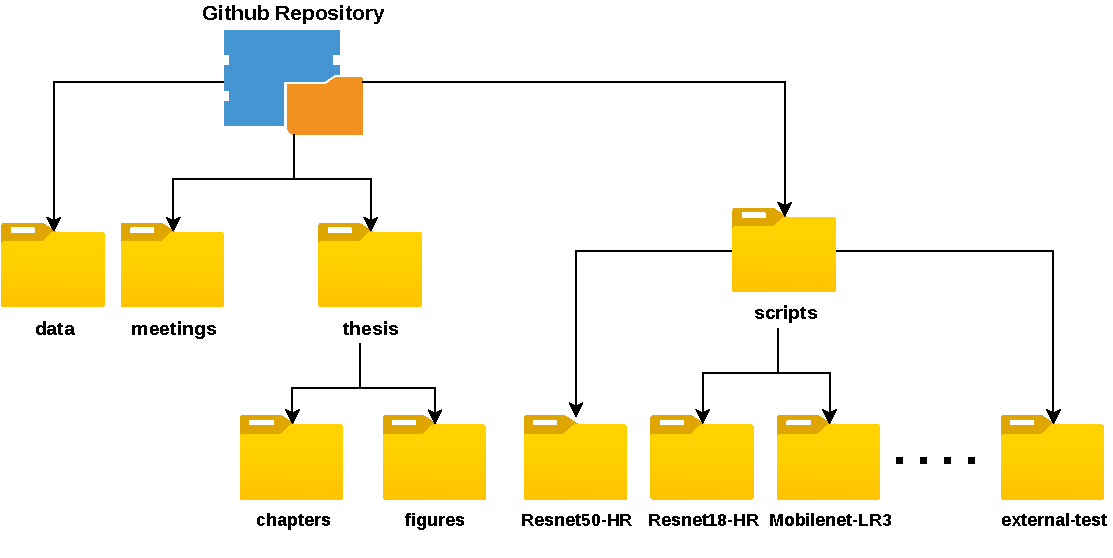
\includegraphics[width=0.88\textwidth]{figures/github-repo.pdf}
    }
    \caption{Overview of the GitHub repository structure.}
    \label{fig:github_structure}
\end{figure}

\FloatBarrier

The different experiments were organised in separate folders. Each of the eight main experiments contains the corresponding \textbf{dataset.py}, \textbf{train.py}, \textbf{test.py}, \textbf{labels.csv}, and the generated experiment outputs. Once an experiment was completed, its folder was kept unchanged so that later modifications did not affect already finished experiments. The Grad-CAM and Grad-CAM++ scripts were stored inside the corresponding experiment folders, while the external Uganda test was kept separately in its own \textbf{external-test/} folder.

Not all paths were handled in exactly the same way. For example, in \textbf{gradcam.py}, the dataset path and checkpoint path are defined at the beginning of the script, while other scripts use command-line arguments for some paths. This reflects the way the individual experiment scripts were developed and stored during the project.

An important part of the reproducibility is the fixed dataset split. The \textbf{build\_labels.py} script performs the 70/15/15 split at patient level and uses a fixed random seed of 42. This means that running the script again with the same dataset produces the same patient assignment for training, validation, and testing. The resulting assignments are stored in \textbf{labels.csv} and reused throughout the experiments. Each experiment also keeps its \textbf{best\_model.pth} checkpoint together with its result files and visual outputs. Information about the datasets is additionally documented in a \textbf{README.md} file inside the \textbf{data/} folder. 

There are still some limits to reproducibility. The fixed seed of 42 controls the patient split, but the training scripts do not fix all random operations with a global PyTorch seed. Random data augmentation and model training can therefore produce small differences when an experiment is trained again. The experiments were also executed using the Apple MPS backend, where exact numerical results are not guaranteed to be identical between repeated runs. For this reason, the saved checkpoints and result files are kept together with each completed experiment. In addition, the external image datasets cannot be redistributed with the source code and have to be downloaded separately from their original providers.





















\chapter{Testing and Evaluation}
\label{chap:testing}



\chapter{Benchmarking}
\label{chap:benchmarking}

To have a perspective on where the performance of the developed models stands in the research field, the models are benchmarked against existing published studies that use thick blood smears.

The comparison considers relevant aspects such as the data used, whole-image versus patch-based approaches, and the reported performance metrics. Because the selected studies differ in these aspects, the comparison is indicative and not a ranking of the different methods. Smartphone-based and lightweight approaches are also considered, since they are relevant to the future deployment direction of this project and to the reduced-resolution experiments.

In the following sections, the selected studies will first be presented and then compared with the results of this thesis. At the end of the chapter, the main differences and findings will be discussed.

\section{Selected previous Studies for Comparison}

The selection of the studies for the benchmarking was based on whether they used thick blood smears, deep learning methods, and low-resource or smartphone-based settings. Lightweight models for resource-limited deployment were also given priority. 

Two particularly relevant studies are Kassim et al. \cite{Kassim2021}, published in 2021, and Yang et al. \cite{Yang2020}, published in 2020.

Kassim et al. \cite{Kassim2021} proposed PlasmodiumVF-Net for malaria diagnosis from thick blood smear images. Their system combines parasite detection with classification and was evaluated on a dataset containing P. falciparum, P. vivax, and uninfected samples. This study was selected because it uses the same NLM/NIH dataset family as the dataset used in this thesis and therefore provides one of the closest comparisons.

Yang et al. \cite{Yang2020} developed a smartphone-based deep learning system for parasite detection in thick blood smear images. Their approach combines candidate screening with a CNN and was designed for use on mobile devices. This study is relevant because it combines thick smear microscopy, smartphone image acquisition, and deep learning.

Two other studies were also selected because they share similar aspects with the work in this thesis. These are Maturana et al. \cite{Maturana2023} and Vásquez Ascate et al. \cite{VasquezAscate2026}.

Maturana et al. \cite{Maturana2023} presented the iMAGING system, which combines a low-cost robotized microscope, smartphone image acquisition, and CNN-based parasite detection. Several object detection architectures were compared on thick blood smear images. This study was selected mainly because of its system-level similarity to the future deployment direction of this project.

Vásquez Ascate et al. \cite{VasquezAscate2026} developed a smartphone-based system that detects parasites in thick blood smears using several lightweight object detection models. The dataset was collected from real clinical samples using different smartphone models and included both P. vivax and P. falciparum. This study was selected because it combines thick blood smears, smartphone acquisition, lightweight architectures, and deployment-oriented evaluation.

\section{Comparison with Previous Studies}

Table~\ref{tab:benchmark} summarises the results of this thesis together with the four selected studies. The comparison includes the data used, the architectures, the task, and the main reported results.

\begin{table}[htbp]
\centering
\caption{Comparison with selected previous studies.}
\label{tab:benchmark}
\normalsize
\resizebox{\textwidth}{!}{%
\begin{tabular}{|p{2.7cm}|p{3.8cm}|p{3.6cm}|p{4.0cm}|p{3.6cm}|}
\hline
\textbf{Study} &
\textbf{Data} &
\textbf{Architecture} &
\textbf{Task } &
\textbf{Main Results} \\
\hline

This thesis &
6038 NLM thick-smear images &
ResNet50, ResNet18, MobileNetV3-Small &
Whole-image binary classification &
Best HR accuracy: 99.69\%, MobileNetV3-Small at LR3: 92.76\% \\
\hline

Kassim et al. \cite{Kassim2021} &
Approx. 6000 images, 350 patients &
Mask R-CNN and ResNet50 &
Detection and image/patient-level classification &
83.9\% image-level, 92.3\% patient-level accuracy \\
\hline

Yang et al. \cite{Yang2020} &
1819 images, 150 patients &
Custom CNN &
Patch classification: parasite vs. background &
93.46\% accuracy \\
\hline

Maturana et al. \cite{Maturana2023} &
2571 thick-smear images &
YOLOv5x and other detectors &
Parasite detection &
YOLOv5x: F-score 92.79\% \\
\hline

Vásquez Ascate et al. \cite{VasquezAscate2026} &
8625 images, 400 slides &
YOLOv11n and other lightweight detectors &
Parasite object detection &
YOLOv11n: 90.92\% accuracy, F1 93.8\% \\
\hline

\end{tabular}%
}
\end{table}

\FloatBarrier

The study of Kassim et al. \cite{Kassim2021} provides the closest comparison to this thesis because they use the same NLM/NIH thick-smear dataset family that was used in this work. On top of that, their method also includes ResNet50, which was one of the high-performing architectures during the testing phase. The main difference is that their PlasmodiumVF-Net first detects parasite candidates using Mask R-CNN and then uses ResNet50 to filter false-positive candidates before performing image- and patient-level classification. Their framework reached an overall accuracy of 83.9\% at image level and 92.3\% at patient level. On the other hand, the approach in this thesis directly classifies the complete image as infected or uninfected, with the best full-resolution models reaching 99.69\% image-level accuracy. The higher accuracy in this thesis should be interpreted with care because Kassim et al. distinguish between P. vivax, P. falciparum, and uninfected samples, while this thesis uses a binary infected/uninfected classification.

The study of Yang et al. \cite{Yang2020} also provides a relevant comparison because they use thick blood smear images for smartphone-based malaria detection. Their method first identifies potential parasites using an intensity-based Iterative Global Minimum Screening (IGMS). Then, it uses a customised CNN to classify each candidate as parasite or background. Their CNN reached an accuracy of 93.46\%, a sensitivity of 92.59\% and a specificity of 94.33\%. The deployment-relevant model in this work is MobileNetV3-Small, which provides a useful comparison because Yang et al. target smartphone-based detection and MobileNetV3-Small was selected as the lightweight architecture for the future deployment direction of this thesis. At full resolution, MobileNetV3-Small reached an accuracy of 99.69\%. After the optimisation at LR3, it reached an accuracy of 92.76\%, a sensitivity of 96.40\% and a specificity of 79.31\%. The LR3 accuracy is close to the 93.46\% accuracy reported by Yang et al., although the two approaches solve different tasks. Yang et al. classify regions as parasite or background, while MobileNetV3-Small in this thesis classifies complete images as either infected or uninfected.

The studies by Maturana et al. \cite{Maturana2023} and Vásquez Ascate et al. \cite{VasquezAscate2026} are more focused on parasite detection and practical deployment. Both use object detection models on thick blood smear images and include smartphone-based image acquisition. Maturana et al. used YOLOv5x to detect leukocytes and Plasmodium trophozoites and reached an overall F-score of 92.79\% for this detection task. Vásquez Ascate et al. used YOLOv11n for parasite detection and reached an accuracy of 90.92\% and an F1-score of 93.8\%. MobileNetV3-Small at LR3 in this thesis reached an accuracy of 92.76\% and an F1-score of 95.45\% for the binary classification of complete images as infected or uninfected. The results are quite close in terms of the reported performance metrics. However, these metrics should not be understood in the same way because the models are solving different tasks. Maturana et al. and Vásquez Ascate et al. focus on detecting parasites inside the image, while the model in this thesis classifies the complete image as infected or uninfected.

\section{Discussion of the Results}

The models developed in this work show in general a high performance, especially with full-resolution images, with the best accuracy reaching 99.69\%. This performance is higher than the results reported in all selected studies. However, this does not necessarily mean that the other approaches are inferior, since the tasks and their complexity are different. Binary classification is a simpler task compared with parasite detection or species classification. Even so, the performance achieved during the testing phase still shows that the developed models perform very well on the used dataset.

MobileNetV3-Small, which is the deployment-relevant model in this work, also reached good performance. After the optimisation at LR3, it achieved an accuracy of 92.76\% and a sensitivity of 96.40\%, although the specificity was 79.31\%. This lower specificity may be related to the class imbalance in the dataset, since only 50 uninfected patients were available compared with 300 infected patients. The overall performance is also in a similar range to the deployment-oriented studies discussed in the previous section. This supports the idea that a lightweight model can still maintain good performance when working with reduced image resolution.

As mentioned in the previous chapters, the goal of the overall project to which this work belongs is malaria prescreening. In this context, the achieved sensitivity of 96.40\% at LR3 is positive because most infected images are still detected. On the other hand, the specificity of 79.31\% means that more uninfected images are incorrectly flagged as infected. For a prescreening system, this may be more acceptable than missing infected images, but the number of false-positive predictions should still be improved.

What cannot be proved from this benchmarking is whether one of the compared approaches is generally better than the others. The studies use different datasets, tasks, models, acquisition methods and evaluation metrics. In addition, the reduced-resolution experiments in this thesis were simulated from the available images and were not performed using images captured with the final smartphone and microscope setup.

Overall, the benchmarking with the four selected studies gives a useful indication that the results of this thesis are promising for the malaria prescreening task and that the models can still achieve good performance at lower resolutions. However, an evaluation using images captured with a smartphone and microscope setup is still required to test the performance under real deployment conditions.



\chapter{Conclusion}
\label{chap:conclusion}

The work of this thesis focused on developing a deep learning model for malaria prescreening with limited-resource conditions in mind, including the future use of smartphone-based images. This thesis is part of a larger system that also includes the development of an ocular adapter, which is intended to be attached to a microscope and enable the capture of thick blood smear images using a smartphone. The model developed in this work is intended to classify complete images as infected or uninfected. An important requirement was therefore also the evaluation of lightweight architectures that could later be suitable for deployment.

To achieve the intended goal of this work, the NLM/NIH thick blood smear dataset was selected for training, validation and testing. A patient-based split of 70\% training, 15\% validation and 15\% testing was used. The selected architectures were ResNet50 as the main high-performance reference model, ResNet18 as a smaller ResNet architecture, and MobileNetV3-Small as the deployment-relevant lightweight model. Since the different parts of the overall project were developed in parallel, the final image resolution of the ocular adapter was not yet available during this thesis. For this reason, different resolution levels were simulated, starting from HR at 224 pixels and reducing the image resolution to LR3 at 56 pixels before resizing back to the model input size. This allowed the behaviour of the models under increasingly reduced image resolution to be investigated. Grad-CAM and Grad-CAM++ were also used to analyse which image regions influenced the predictions. In addition to the NLM/NIH test data, an external test using the AIR Uganda dataset was performed to evaluate the models on images with different characteristics from the development dataset.

The testing results showed that all architectures achieved very high performance at full resolution. ResNet50 reached an accuracy of 99.58\% at HR. Its performance remained high at LR1 and LR2, but a clearer decrease was observed at LR3, where the accuracy dropped to 92.86\%. The specificity also decreased to 73.89\%, while the sensitivity remained high at 98.00\%. ResNet18 and MobileNetV3-Small both reached the highest full-resolution accuracy of 99.69\% and a sensitivity of 100\%, meaning that all infected images in the internal test set were correctly classified. Under stronger resolution reduction, the main decrease was seen especially in the classification of uninfected images, with more false-positive predictions being produced. MobileNetV3-Small was therefore further optimised at LR3 and finally reached an accuracy of 92.76\%, a sensitivity of 96.40\%, a specificity of 79.31\% and an F1-score of 95.45\%.

The Grad-CAM and Grad-CAM++ results raised more questions about the behaviour of the models. In several examples, strong activations were visible around the edges and dark background of the microscope field instead of only inside the blood smear region. This raised the possibility that the models may partly use image characteristics that are not directly related to the parasites. To further investigate this, the external AIR Uganda dataset was used because its images have different visual characteristics compared with the NLM/NIH dataset. Since this dataset contains only infected images, only the sensitivity could be evaluated. ResNet50 reached a sensitivity of 100\% at HR and 98.48\% at LR3, with only 18 infected images missed at LR3. MobileNetV3-Small reached a sensitivity of 95.60\% at LR3, while ResNet18 showed a lower sensitivity of 82.32\% with 209 false-negative predictions. These results support that the models are not relying only on the specific borders or background characteristics of the NLM/NIH images. However, shortcut learning cannot be completely excluded. The external test also cannot show whether the models tend to predict the infected class when uncertain, because no uninfected samples were available in the AIR Uganda dataset.

Overall, the whole-image classification approach is technically promising based on the results of this work and the comparison with previous studies. Even when the image resolution was strongly reduced, good performance was still achieved. MobileNetV3-Small was the most relevant architecture for future deployment and also showed good performance at both high and low resolution. 

The work of this thesis should be understood as a research prototype for future development and is not yet clinically validated for real-life malaria prescreening. The next important step is to obtain images captured with the combination of the developed ocular adapter, microscope and smartphone. These images will provide the real image resolution and characteristics that can be expected during future deployment. The models can then be tested using real captured images instead of only simulated resolution reductions. Future testing should also include more external datasets, especially datasets containing uninfected images, since this remained an open question during the testing phase. This would allow the specificity and false-positive behaviour of the models to be evaluated more reliably. In addition, using more uninfected samples during future model development could potentially help reduce the number of uninfected images that are incorrectly classified as infected.

A possible future extension of the system could also be parasite detection. After the binary prescreening approach has been further evaluated and improved, the system could be extended to identify parasites inside the image and later also distinguish between different Plasmodium species.


% -------------------------------------------------
% Bibliography
% -------------------------------------------------

\clearpage

\bibliographystyle{IEEEtran}
\bibliography{references}

\end{document}